\documentclass{standalone}
\usepackage{pgfplots}
\begin{document}
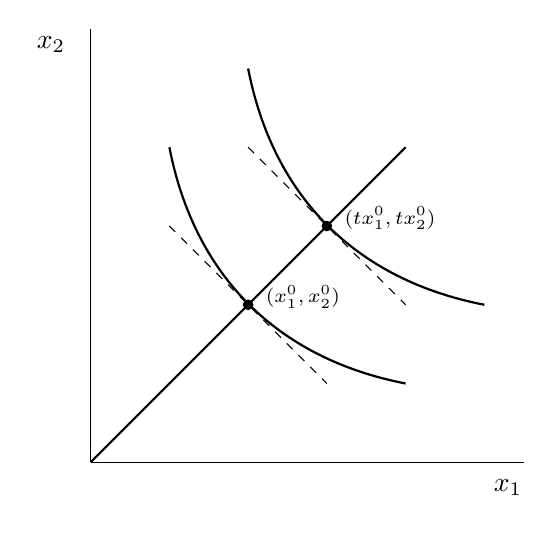
\begin{tikzpicture}
\draw (0,0) -- (5.5,0);
\draw (0,0) -- (0,5.5);
\node[left] at (-0.2,5.3) {$x_2$};
\node[below] at (5.3,-0.1) {$x_1$};
\draw [thick] (1,4) to [out = 281, in = 169] (4,1);
\draw [thick] (2,5) to [out = 281, in = 169] (5,2); 
\draw[dashed] (1,3) -- (3,1);
\draw[dashed] (2,4) -- (4,2);
\draw[thick] (0,0) -- (4,4);
\draw[fill] (2,2) circle [radius = 0.06];
\draw[fill] (3,3) circle [radius = 0.06];
\node[right] at (2.1,2.1) {\scriptsize $(x_1^0, x_2^0)$};
\node[right] at (3.1,3.1) {\scriptsize $(tx_1^0, tx_2^0)$};
\end{tikzpicture}
\end{document}